% Provenance (never printed): cycle 4 SVT, "La planete Terre": earthquakes,
% faults, seismic waves and their recording, magnitude and intensity, the
% link with plate boundaries; natural hazards (tsunamis) and prevention; see
% sources/book1/PROVENANCE.md. Book 1, grade 7, chapter 3.
% Vocabulary guard: P and S waves are named in prose only (they were named in
% g6.4, defined in Book 2 g11); "sediment" not before g7.4; "intensity" is
% always the earthquake's (homograph with physics: linker STOP list).
\chapter{Gempa Bumi}\label{ch:g7:earthquakes}

Pada pagi hari tanggal 26~Desember 2004, di bawah \omterm{def:g2:water-on-earth:ocean}{laut} di lepas ujung barat
laut Sumatra, di Indonesia, \omterm{def:g3:stones-pebbles-sand:rock}{batuan} patah di sepanjang sebuah \omterm{def:g7:earthquakes:fault}{sesar}: itulah
salah satu \omterm{def:g4:volcanoes-earthquakes-first-look:earthquake}{gempa bumi} terbesar yang pernah diukur. Di pantai Sumatra yang
terdekat, \omterm{def:g2:water-on-earth:ocean}{laut} naik dalam gelombang setinggi sampai \qty{51}{m}, yang
menyapu daratan sejauh \qty{5}{km} ke pedalaman. Dalam jam-jam berikutnya,
gelombang itu menyeberangi \omterm{def:g2:water-on-earth:ocean}{Samudra} Hindia dan menghantam pantai lima belas
negara, sampai sejauh Afrika. Kira-kira 230\,000 orang meninggal. Pada waktu
itu, belum ada sistem peringatan di \omterm{def:g2:water-on-earth:ocean}{Samudra} Hindia.
% ledger: usgs:largest, nws:tsunami-2004

\begin{omfigure}
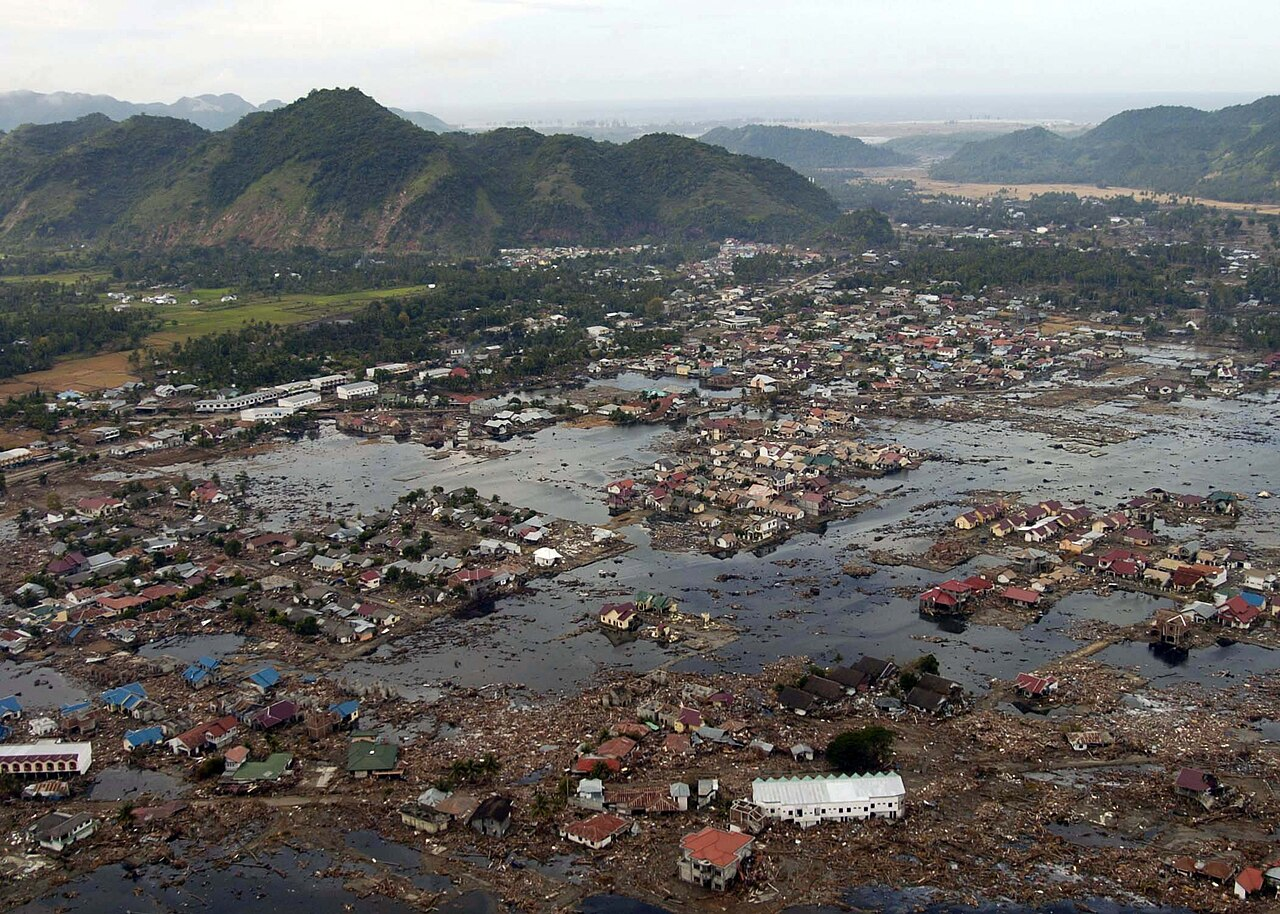
\includegraphics[width=0.78\linewidth]{images/book1/g7-tsunami-village.jpg}

{\small Sebuah desa di dekat pantai Sumatra seminggu sesudah \omterm{def:g7:earthquakes:tsunami}{tsunami} tanggal
26~Desember 2004. Foto Angkatan \omterm{def:g2:water-on-earth:ocean}{Laut} Amerika Serikat karya Philip~A.
McDaniel (domain publik, melalui Wikimedia Commons).}
% ledger: commons:tsunami-village
\label{fig:g7:earthquakes:tsunami-village}
\end{omfigure}

Bagaimana \omterm{def:g3:stones-pebbles-sand:rock}{batuan} patah? Bagaimana para ilmuwan mengetahui, dalam beberapa
menit, di mana sebuah \omterm{def:g4:volcanoes-earthquakes-first-look:earthquake}{gempa bumi} terjadi dan seberapa besar gempa itu? Dan
mengapa \omterm{def:g2:water-on-earth:ocean}{laut}, berjam-jam kemudian, naik di pantai-pantai yang tidak
merasakan apa-apa?

\begin{recall}
Yang disebut \emph{\omterm{def:g4:volcanoes-earthquakes-first-look:earthquake}{gempa bumi}} adalah guncangan tanah yang tiba-tiba, yang
disebabkan oleh \omterm{def:g3:stones-pebbles-sand:rock}{batuan} yang patah dan bergeser, jauh di bawah tanah
(\cref{ch:g4:volcanoes-earthquakes-first-look}). Cangkang luar Bumi terdiri
atas \omterm{def:g7:plate-tectonics:plate}{lempeng-lempeng}, dan 92~\% \omterm{def:g4:volcanoes-earthquakes-first-look:earthquake}{gempa bumi} besar terjadi kurang dari
\qty{300}{km} dari \omterm{def:g7:plate-tectonics:plate-boundary}{batas lempeng} (\cref{ch:g7:plate-tectonics}). Ketika
\omterm{def:g4:volcanoes-earthquakes-first-look:earthquake}{gempa bumi} terjadi, gelombang merambat melalui \omterm{def:g3:stones-pebbles-sand:rock}{batuan} di seluruh Bumi: satu
jenis yang lebih cepat (gelombang~P) dan satu jenis yang lebih lambat
(gelombang~S); dengan mengukur waktu tibanya, para ilmuwan menemukan \omterm{def:g6:inside-the-earth:layers}{inti}
Bumi (\cref{ch:g6:inside-the-earth}).
\end{recall}

\section{Batuan yang patah}

\omterm{def:g7:plate-tectonics:plate}{Lempeng-lempeng} bergerak beberapa sentimeter setahun, tetapi tepinya kasar:
tepi-tepi itu saling melekat sementara bagian lain \omterm{def:g7:plate-tectonics:plate}{lempeng} terus bergerak.
\omterm{def:g3:stones-pebbles-sand:rock}{Batuan} di dekat tepi itu melengkung sedikit, seperti penggaris yang kamu
tekan di kedua ujungnya, dan menyimpan energi. Ketika dorongan itu akhirnya
mengalahkan gesekan, \omterm{def:g3:stones-pebbles-sand:rock}{batuan} itu serentak terlepas dan bergeser: pergeseran
yang tiba-tiba itulah \omterm{def:g4:volcanoes-earthquakes-first-look:earthquake}{gempa bumi}.
% ledger: usgs:eq-basics

\begin{definition}[Sesar]\label{def:g7:earthquakes:fault}
Yang disebut \emph{sesar}\index{sesar} adalah rekahan pada \omterm{def:g3:stones-pebbles-sand:rock}{batuan}, yang di
sepanjangnya kedua bongkah di kedua sisinya telah bergerak terhadap satu
sama lain. Ketika \omterm{def:g4:volcanoes-earthquakes-first-look:earthquake}{gempa bumi}, bongkah-bongkah itu tiba-tiba bergeser di
sepanjang sesar; makin besar sesar dan pergeserannya, makin besar \omterm{def:g4:volcanoes-earthquakes-first-look:earthquake}{gempa
buminya}.
\end{definition}

\omterm{def:g7:plate-tectonics:plate-boundary}{Batas lempeng} terdiri atas banyak \omterm{def:g7:earthquakes:fault}{sesar}, dan sebagian besar \omterm{def:g4:volcanoes-earthquakes-first-look:earthquake}{gempa bumi} di
dunia terjadi pada \omterm{def:g7:earthquakes:fault}{sesar-sesar} itu. Tetapi \omterm{def:g7:earthquakes:fault}{sesar} juga ada di dalam
\omterm{def:g7:plate-tectonics:plate}{lempeng}, dan sebagian di antaranya dapat patah juga. Ketika sebuah \omterm{def:g7:earthquakes:fault}{sesar}
besar patah di dekat permukaan, pergeserannya dapat terlihat di tanah:
sebuah undakan di ladang, jalan yang terpotong menjadi dua, pagar atau
deretan pohon yang bergeser ke samping.
% ledger: usgs:eq-basics

\begin{omfigure}
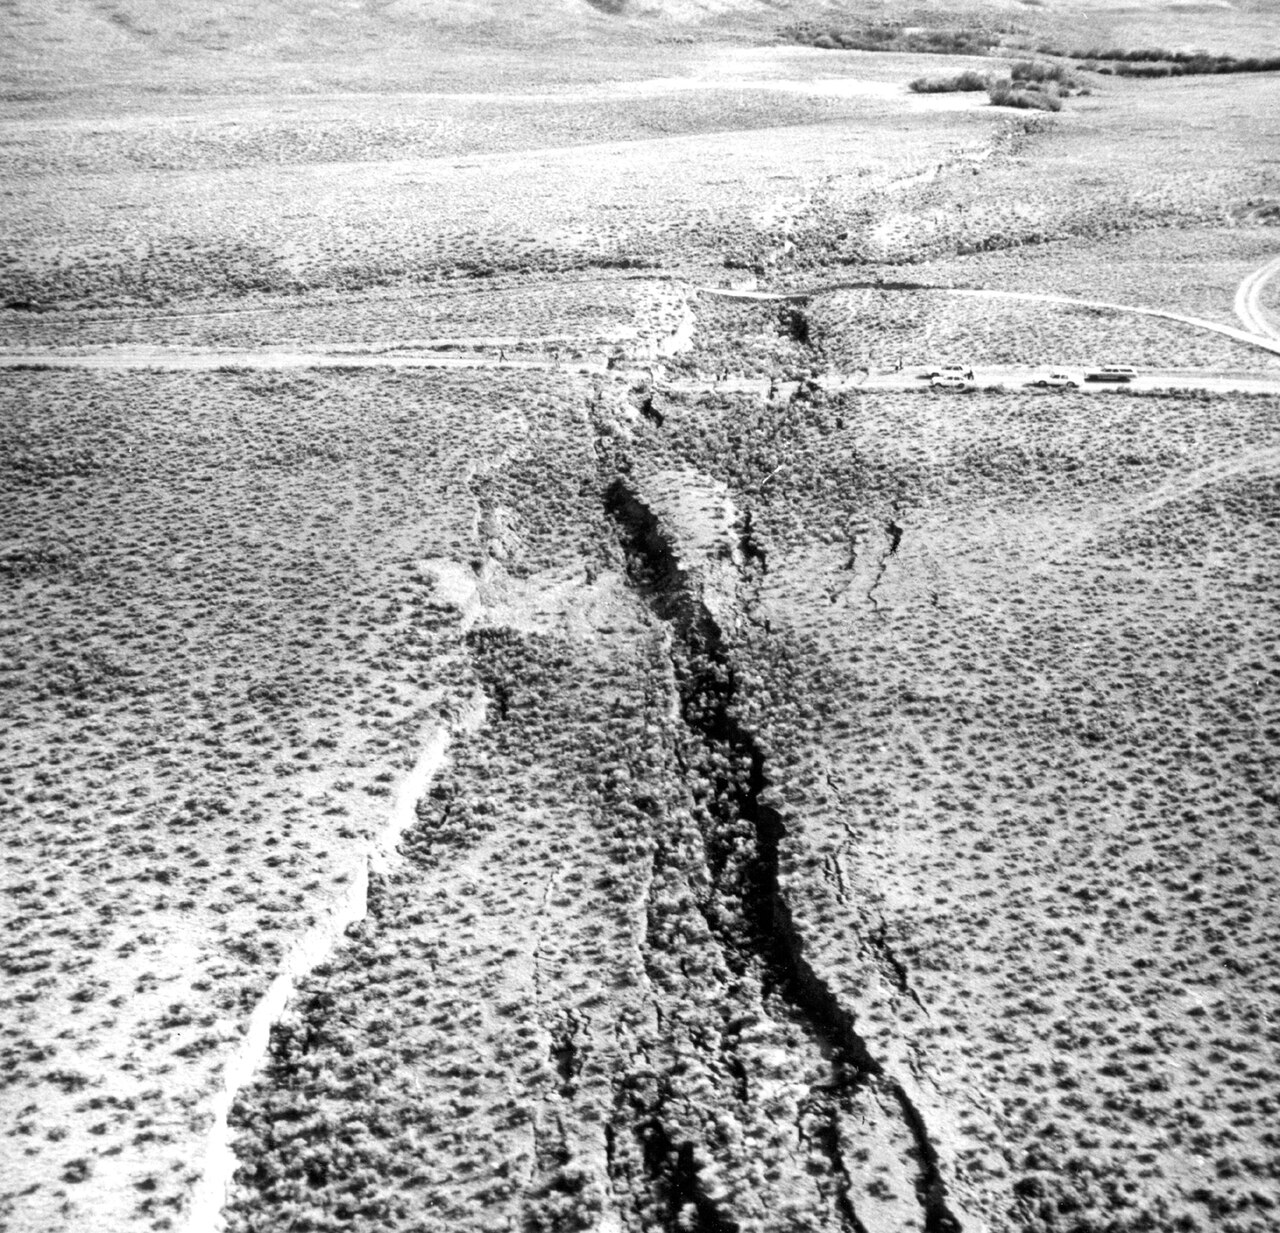
\includegraphics[width=0.62\linewidth]{images/book1/g7-borah-scarp.jpg}

{\small Undakan-undakan di tanah yang ditinggalkan \omterm{def:g4:volcanoes-earthquakes-first-look:earthquake}{gempa bumi} Borah Peak
tahun 1983, di Idaho (Amerika Serikat), dilihat dari udara: di sepanjang
\omterm{def:g7:earthquakes:fault}{sesar}, satu sisi turun terhadap sisi yang lain, dan undakan itu memotong
jalan di bagian atas. Foto: R.~E. Wallace, U.S. Geological Survey (domain
publik, melalui Wikimedia Commons).}
% ledger: commons:borah-scarp
\label{fig:g7:earthquakes:borah}
\end{omfigure}

\begin{definition}[Hiposentrum dan episentrum]\label{def:g7:earthquakes:focus}
Yang disebut \emph{hiposentrum}\index{hiposentrum} sebuah \omterm{def:g4:volcanoes-earthquakes-first-look:earthquake}{gempa bumi} adalah
tempat di bawah tanah, pada \omterm{def:g7:earthquakes:fault}{sesar}, tempat pergeseran dimulai. Yang disebut
\emph{episentrum}\index{episentrum} adalah titik di permukaan Bumi yang
terletak tepat di atas hiposentrum.
\end{definition}

\omterm{def:g7:earthquakes:focus}{Hiposentrum} sering terletak beberapa kilometer sampai beberapa puluh
kilometer di bawah permukaan. Dari 7\,031 \omterm{def:g4:volcanoes-earthquakes-first-look:earthquake}{gempa bumi} \omterm{def:g7:earthquakes:magnitude}{bermagnitudo}~6 atau
lebih yang tercatat antara tahun 1976 dan 2025, 5\,561 --- 79~\% ---
\omterm{def:g7:earthquakes:focus}{hiposentrumnya} kurang dari \qty{70}{km} di bawah permukaan. Tetapi 483 gempa
dimulai lebih dari \qty{300}{km} di bawah permukaan, dan yang terdalam
\qty{688}{km}: gempa-gempa bumi dalam ini terjadi di tempat satu \omterm{def:g7:plate-tectonics:plate}{lempeng}
menunjam ke bawah \omterm{def:g7:plate-tectonics:plate}{lempeng} lain, di dalam \omterm{def:g7:plate-tectonics:plate}{lempeng} yang menunjam itu.
% ledger: data:usgs-comcat (figdata/grade-7/quake_counts.py, part depth)

\omterm{def:g4:volcanoes-earthquakes-first-look:earthquake}{Gempa bumi} besar jarang datang sendirian. Gempa itu sering diikuti oleh
gempa-gempa yang lebih kecil di tempat yang sama, yaitu \emph{gempa
susulan}, selama berminggu-minggu, berbulan-bulan, bahkan bertahun-tahun.
Kadang-kadang gempa-gempa yang lebih kecil datang sebelumnya, tetapi tidak
ada yang dapat mengetahui bahwa gempa-gempa itu peringatan sampai gempa
yang besar terjadi: para ilmuwan tidak dapat meramalkan \omterm{def:g4:volcanoes-earthquakes-first-look:earthquake}{gempa bumi}. Mereka
hanya dapat mengatakan \omterm{def:g7:earthquakes:fault}{sesar} mana yang suatu hari akan patah lagi, dan
membantu orang bersiap-siap.
% ledger: usgs:eq-basics, usgs:seismograph

\begin{omfigure}
\begin{tikzpicture}[font=\small, x=1cm, y=1cm]
  % a block of crust seen in perspective: front face and top face
  \def\dx{2.2}\def\dy{1.3}
  % top surface: two blocks separated by the fault trace
  \fill[green!12] (0,0) -- (4.6,0) -- (4.6+\dx,\dy) -- (\dx,\dy) -- cycle;
  \fill[green!18] (4.6,0) -- (9,0) -- (9+\dx,\dy) -- (4.6+\dx,\dy) -- cycle;
  % front face
  \fill[brown!30] (0,0) -- (4.6,0) -- (3.4,-4) -- (0,-4) -- cycle;
  \fill[brown!40] (4.6,0) -- (9,0) -- (9,-4) -- (3.4,-4) -- cycle;
  % right face
  \fill[brown!22] (9,0) -- (9+\dx,\dy) -- (9+\dx,\dy-4) -- (9,-4) -- cycle;
  % fault plane on the front face and trace on top
  \draw[very thick, red!70!black] (4.6,0) -- (3.4,-4);
  \draw[very thick, red!70!black] (4.6,0) -- (4.6+\dx,\dy);
  % slip arrows
  \draw[-{Stealth[length=2.5mm]}, thick] (2.6,-0.35) -- (1.6,-0.35);
  \draw[-{Stealth[length=2.5mm]}, thick] (6.4,-0.35) -- (7.4,-0.35);
  \node[font=\footnotesize, anchor=south] at (2.1,-0.3) {bongkah 1};
  \node[font=\footnotesize, anchor=south] at (6.9,-0.3) {bongkah 2};
  % focus and waves
  \coordinate (F) at (3.95,-2.4);
  \foreach \r in {0.5,1.0,1.5,2.0}
    \draw[blue!60, dashed] (F) circle (\r);
  \fill[red!80!black] (F) circle (0.13);
  % epicentre: on the surface, straight above the focus (front edge of the top face)
  \coordinate (E) at (3.95,0);
  \draw[black!60, densely dotted, thick] (F) -- (E);
  \node[star, star points=5, star point ratio=2.4, fill=orange, draw=black, inner sep=1.4pt] at (E) {};
  % labels
  \node[anchor=west] at (9.5,-2.3) {hiposentrum};
  \draw[black!60] (9.45,-2.3) -- (4.1,-2.4);
  \node[anchor=south west] at (4.9,1.9) {episentrum};
  \draw[black!60] (4.95,1.95) -- (4.05,0.12);
  \node[anchor=south, red!70!black] at (6.8,1.3) {sesar};
  \node[anchor=east, blue!60!black, align=right] at (-0.15,-2.6) {gelombang\\menyebar ke\\segala arah};
  \draw[blue!60, -{Stealth}] (-0.1,-2.6) -- (1.9,-2.5);
\end{tikzpicture}

{\small \omterm{def:g7:earthquakes:fault}{Sesar}, \omterm{def:g7:earthquakes:focus}{hiposentrum}, dan \omterm{def:g7:earthquakes:focus}{episentrum} (gambar, tidak berskala). Kedua
bongkah saling bergeser di sepanjang \omterm{def:g7:earthquakes:fault}{sesar} (merah); pergeseran dimulai di
\omterm{def:g7:earthquakes:focus}{hiposentrum}, dan gelombang menyebar darinya ke segala arah, seperti riak di
kolam. \omterm{def:g7:earthquakes:focus}{Episentrum} (bintang) terletak di permukaan, tepat di atas
\omterm{def:g7:earthquakes:focus}{hiposentrum}.}
% ledger: usgs:eq-basics
\label{fig:g7:earthquakes:fault}
\end{omfigure}


\section{Merekam gempa bumi}

\begin{definition}[Seismometer dan seismogram]\label{def:g7:earthquakes:seismometer}
Yang disebut \emph{seismometer}\index{seismometer} adalah alat yang merekam
guncangan tanah. Rekamannya, sebuah garis berkelok-kelok yang digambar
terhadap waktu, disebut \emph{seismogram}\index{seismogram}.
\end{definition}

Gagasan \omterm{def:g7:earthquakes:seismometer}{seismometer} itu sederhana. Sebuah rangka dipasang kuat-kuat pada
tanah; sebuah beban berat digantungkan padanya dengan pegas. Ketika tanah
berguncang, rangka ikut berguncang, tetapi beban yang berat itu, yang hanya
ditahan oleh pegasnya, hampir tetap diam. Alat itu merekam gerak rangka
terhadap beban yang diam: itulah gerak tanah. Pada gambar di bawah ini,
sebuah pena yang dipasang pada beban menggambarkannya pada kertas yang
dililitkan pada sebuah tromol yang berputar.
% ledger: usgs:seismograph

\begin{omfigure}
\begin{tikzpicture}[font=\small, x=1cm, y=1cm]
  \begin{scope}
    % ground
    \fill[brown!30] (-0.6,-0.6) rectangle (5.0,0);
    \draw[decorate, decoration={snake, amplitude=1.2pt, segment length=6pt}, brown!70!black, thick]
      (-0.6,0) -- (5.0,0);
    % frame
    \fill[black!55] (0,0) rectangle (0.25,3.2);
    \fill[black!55] (0,3.0) rectangle (2.4,3.25);
    % spring and weight
    \draw[decorate, decoration={coil, aspect=0.5, segment length=3pt, amplitude=4pt}, thick]
      (2.1,3.0) -- (2.1,2.1);
    \fill[black!80] (1.7,1.45) rectangle (2.5,2.1);
    \node[white, font=\scriptsize] at (2.1,1.78) {beban};
    % pen arm and drum
    \draw[thick] (2.5,1.75) -- (3.45,1.75);
    \fill (3.45,1.75) circle (0.05);
    \draw[thick, fill=white] (3.95,1.75) circle (0.5);
    \draw[thick] (3.95,1.25) -- (3.95,0);
    \draw[-{Stealth}, black!60] (4.55,2.2) arc (40:-40:0.7);
    % labels
    \node[anchor=east, align=right, font=\footnotesize] at (-0.1,2.3) {rangka yang\\dipasang\\pada tanah};
    \node[anchor=west, font=\footnotesize] at (2.6,2.65) {pegas};
    \draw[black!60] (2.55,2.65) -- (2.25,2.6);
    \node[anchor=north, align=center, font=\footnotesize] at (2.1,1.35) {beban berat:\\tetap diam};
    \node[anchor=west, align=left, font=\footnotesize] at (4.7,1.05) {tromol\\kertas\\berputar};
    \node[anchor=north, font=\footnotesize] at (2.2,-0.65) {tanah berguncang};
  \end{scope}
  \begin{scope}[xshift=7.2cm, yshift=0.4cm]
    \begin{axis}[width=7.6cm, height=4.2cm, xmin=0, xmax=60, ymin=-1.1, ymax=1.1,
        axis x line=bottom, axis y line=none, xlabel={waktu (detik)},
        tick label style={font=\scriptsize}, label style={font=\footnotesize}, clip=false]
      \addplot[black, line width=0.4pt] table[x=t, y=v] {figdata/out/grade-7-epicentre-m-trace.dat};
      \draw[blue!70!black, -{Stealth[length=2mm]}] (axis cs:10,1.45) -- (axis cs:10,0.45);
      \node[blue!70!black, font=\scriptsize, anchor=south east, align=right] at (axis cs:10.5,1.45) {gelombang yang\\lebih cepat tiba};
      \draw[red!70!black, -{Stealth[length=2mm]}] (axis cs:20,1.45) -- (axis cs:20,1.05);
      \node[red!70!black, font=\scriptsize, anchor=south west, align=left] at (axis cs:19.5,1.45) {gelombang yang\\lebih lambat tiba};
      \draw[{Stealth[length=2mm]}-{Stealth[length=2mm]}] (axis cs:10,-0.75) -- (axis cs:20,-0.75);
      \node[font=\scriptsize, anchor=east] at (axis cs:9,-0.75) {selisih: 10 s};
    \end{axis}
  \end{scope}
\end{tikzpicture}

{\small Kiri: prinsip kerja \omterm{def:g7:earthquakes:seismometer}{seismometer} (gambar). Kanan: \omterm{def:g7:earthquakes:seismometer}{seismogram} yang
digambar untuk buku ini (bukan rekaman yang sesungguhnya): garisnya
tenang, lalu gelombang yang lebih cepat tiba, lalu, sepuluh detik kemudian,
gelombang yang lebih lambat dan lebih besar.}
% ledger: usgs:seismograph (trace drawn by figdata/grade-7/epicentre.py, part m-trace)
\label{fig:g7:earthquakes:seismometer}
\end{omfigure}

\subsection*{Seberapa jauh gempa bumi itu?}

\omterm{def:g7:earthquakes:seismometer}{Seismogram} menceritakan lebih banyak daripada ``tanah berguncang''.
Gelombang yang lebih cepat selalu tiba lebih dahulu dan yang lebih lambat
sesudahnya. Di dekat \omterm{def:g7:earthquakes:focus}{hiposentrum}, keduanya tiba hampir bersamaan; di tempat
yang jauh, gelombang yang lebih lambat makin lama makin tertinggal, sama
seperti ketika \omterm{def:g5:natural-hazards:storm}{badai}, guntur makin jauh tertinggal di belakang kilat jika
\omterm{def:g5:natural-hazards:storm}{badainya} jauh. Jadi selisih waktu antara kedua kedatangan itu menunjukkan
jarak ke \omterm{def:g4:volcanoes-earthquakes-first-look:earthquake}{gempa bumi}.
% ledger: usgs:seismograph

Berapa kilometer untuk setiap detik selisih? Hal itu bergantung pada
kecepatan kedua gelombang di dalam \omterm{def:g3:stones-pebbles-sand:rock}{batuan} yang dilaluinya. Dengan kecepatan
dari model acuan Bumi (\cref{ch:g6:inside-the-earth}), setiap detik selisih
berarti kira-kira \qty{7}{km} di \omterm{def:g6:inside-the-earth:layers}{kerak} atas dan \qty{9}{km} di \omterm{def:g6:inside-the-earth:layers}{kerak} bawah.
Dalam latihan-latihan bab ini kita memakai nilai bulat \qty{8}{km} untuk
setiap detik.
% ledger: data:prem (computed in figdata/grade-7/epicentre.py, part rule)

\begin{method}[Menemukan episentrum dengan tiga stasiun]\label{met:g7:earthquakes:three-circles}
\begin{enumerate}
  \item Pada \omterm{def:g7:earthquakes:seismometer}{seismogram} setiap stasiun, bacalah selisih waktu antara
        kedatangan gelombang yang lebih cepat dan kedatangan gelombang yang
        lebih lambat.
  \item Ubahlah setiap selisih menjadi jarak (di sini: $8 \times$ selisih
        dalam detik, dalam kilometer).
  \item Pada \omterm{def:g2:drawing-to-map:map}{peta}, gambarlah di sekeliling setiap stasiun sebuah lingkaran
        yang jari-jarinya sama dengan jaraknya. \omterm{def:g7:earthquakes:focus}{Episentrum} terletak di suatu
        tempat pada setiap lingkaran.
  \item Dengan dua lingkaran, biasanya ada dua titik yang mungkin; lingkaran
        ketiga hanya melalui salah satunya: itulah \omterm{def:g7:earthquakes:focus}{episentrumnya}.
\end{enumerate}
\end{method}

\begin{example}[Tiga lingkaran]\label{ex:g7:earthquakes:three-circles}
Tiga stasiun merekam \omterm{def:g4:volcanoes-earthquakes-first-look:earthquake}{gempa bumi} yang sama. Selisihnya \qty{10}{s} di
stasiun~M1, \qty{11.25}{s} di M2, dan \qty{9.75}{s} di M3. Jaraknya
$8 \times 10 = \qty{80}{km}$, $8 \times 11.25 = \qty{90}{km}$, dan
$8 \times 9.75 = \qty{78}{km}$. Ketiga lingkaran itu, yang digambar di bawah
ini, bertemu di satu titik saja: \omterm{def:g7:earthquakes:focus}{episentrum}.
% ledger: usgs:seismograph (figdata/grade-7/epicentre.py, parts m-stations and m-circles)
\end{example}

\begin{omfigure}
\begin{tikzpicture}
  \begin{axis}[axis equal image, width=8.2cm, xmin=-150, xmax=170, ymin=-160, ymax=160,
      xtick={-120,-80,...,160}, ytick={-120,-80,...,120}, grid=both, grid style={black!12},
      tick label style={font=\scriptsize}, xlabel={km}, ylabel={km}, label style={font=\footnotesize}]
    \addplot[blue!60!black, line width=0.6pt] table[x=x, y=y] {figdata/out/grade-7-epicentre-m-circles.dat};
    \addplot[only marks, mark=triangle*, mark size=3pt, black,
        nodes near coords, point meta=explicit symbolic,
        nodes near coords style={font=\scriptsize, anchor=north, yshift=-2pt}]
      table[x=x, y=y, meta=name] {figdata/out/grade-7-epicentre-m-stations.dat};
    \node[star, star points=5, star point ratio=2.4, fill=orange, draw=black, inner sep=1.6pt] at (axis cs:0,0) {};
    \draw[black!60] (axis cs:-4,-4) -- (axis cs:-60,-75);
    \node[font=\scriptsize, anchor=north east, inner sep=1pt] at (axis cs:-60,-75) {episentrum};
  \end{axis}
\end{tikzpicture}

{\small Setiap lingkaran berpusat di sebuah stasiun (segitiga), dengan
jari-jari yang sama dengan jarak stasiun itu ke \omterm{def:g4:volcanoes-earthquakes-first-look:earthquake}{gempa bumi}. Ketiga
lingkaran itu hanya bertemu di satu titik, yaitu \omterm{def:g7:earthquakes:focus}{episentrum} (bintang).}
% ledger: usgs:seismograph (figdata/grade-7/epicentre.py, parts m-stations and m-circles)
\label{fig:g7:earthquakes:three-circles}
\end{omfigure}

\begin{omfigure}
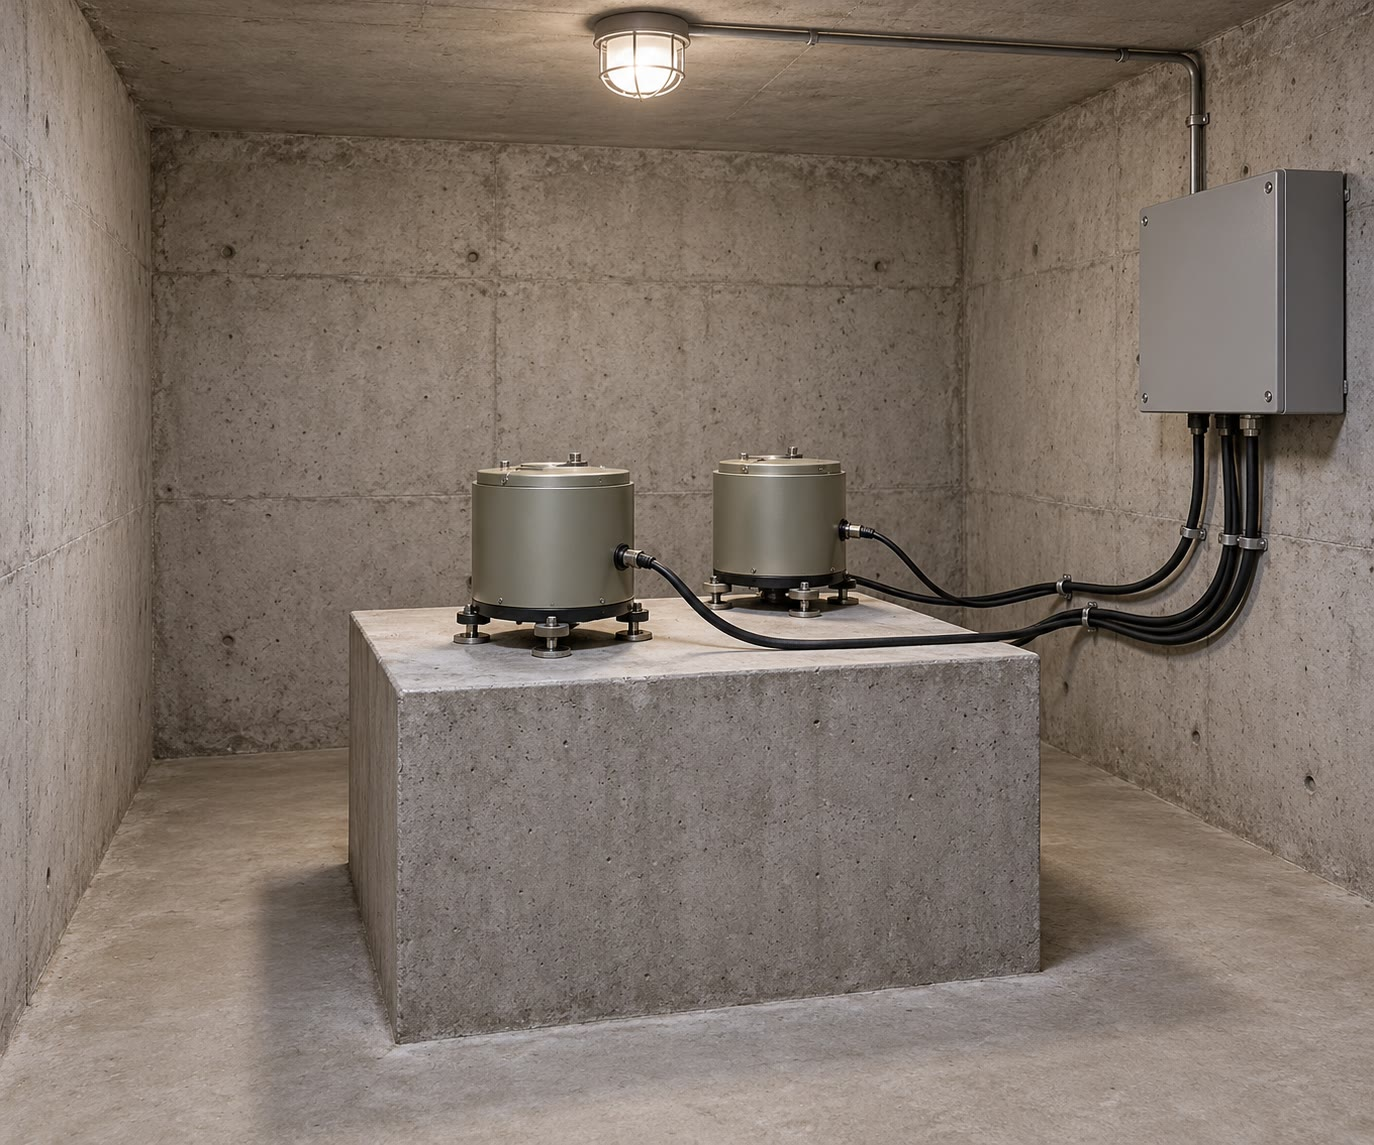
\includegraphics[width=0.58\linewidth]{images/book1/ai/g7-seismometer-vault.jpg}

{\small \omterm{def:g7:earthquakes:seismometer}{Seismometer-seismometer} di sebuah ruang bawah tanah yang sunyi,
diletakkan di atas tiang beton yang bertumpu pada \omterm{def:g3:stones-pebbles-sand:rock}{batuan}, jauh dari jalan
dan mesin (ilustrasi AI dari suatu adegan umum).}
\label{fig:g7:earthquakes:vault}
\end{omfigure}

\section{Seberapa besar? Magnitudo dan intensitas}

Dua bilangan yang berbeda menggambarkan sebuah \omterm{def:g4:volcanoes-earthquakes-first-look:earthquake}{gempa bumi}, dan keduanya sering tertukar.

\begin{definition}[Magnitudo]\label{def:g7:earthquakes:magnitude}
Yang disebut \emph{magnitudo}\index{magnitudo} sebuah \omterm{def:g4:volcanoes-earthquakes-first-look:earthquake}{gempa bumi} adalah
ukuran besarnya: energi yang dilepaskan di sumbernya. Magnitudo dihitung
dari \omterm{def:g7:earthquakes:seismometer}{seismogram}. Setiap \omterm{def:g4:volcanoes-earthquakes-first-look:earthquake}{gempa bumi} mempunyai satu magnitudo saja, yang
ditulis dengan satu tempat desimal, misalnya 6.3 atau 9.1.
\end{definition}

\begin{definition}[Intensitas]\label{def:g7:earthquakes:intensity}
Yang disebut \emph{intensitas}\index{intensitas} sebuah \omterm{def:g4:volcanoes-earthquakes-first-look:earthquake}{gempa bumi} di suatu
tempat menggambarkan seberapa kuat tanah berguncang di sana, berdasarkan apa
yang dirasakan orang dan kerusakan yang mereka lihat. Intensitas ditulis
dengan angka Romawi, dari I (tidak terasa) sampai XII (kehancuran total).
Satu \omterm{def:g4:volcanoes-earthquakes-first-look:earthquake}{gempa bumi} mempunyai banyak intensitas: berbeda di setiap tempat.
\end{definition}

Skala magnitudo naik dengan cepat. Setiap langkah 1 pada \omterm{def:g7:earthquakes:magnitude}{magnitudo} berarti
gelombang yang kira-kira 10~kali lebih besar pada \omterm{def:g7:earthquakes:seismometer}{seismogram} dan energi
yang dilepaskan kira-kira 32~kali lebih banyak. \omterm{def:g4:volcanoes-earthquakes-first-look:earthquake}{Gempa bumi} \omterm{def:g7:earthquakes:magnitude}{bermagnitudo}~8
melepaskan energi kira-kira $32 \times 32 \approx 1000$ kali lebih banyak
daripada gempa \omterm{def:g7:earthquakes:magnitude}{bermagnitudo}~6.
% ledger: usgs:mag-energy

\begin{method}[Membandingkan dua magnitudo]\label{met:g7:earthquakes:magnitudes}
Untuk membandingkan energi dua \omterm{def:g4:volcanoes-earthquakes-first-look:earthquake}{gempa bumi}, hitunglah langkah-langkah utuh
di antara \omterm{def:g7:earthquakes:magnitude}{magnitudonya}, dan kalikan dengan 32 satu kali untuk setiap
langkah: 1~langkah, 32~kali; 2~langkah, kira-kira 1000~kali; 3~langkah,
kira-kira 32\,000~kali.
\end{method}

\begin{example}[Magnitudo 9 dan magnitudo 7]\label{ex:g7:earthquakes:nine-seven}
\omterm{def:g4:volcanoes-earthquakes-first-look:earthquake}{Gempa bumi} tahun 2004 di lepas pantai Sumatra \omterm{def:g7:earthquakes:magnitude}{bermagnitudo} 9.1. \omterm{def:g4:volcanoes-earthquakes-first-look:earthquake}{Gempa bumi}
\omterm{def:g7:earthquakes:magnitude}{bermagnitudo}~7.1 dua langkah lebih kecil: gempa itu melepaskan energi
$32 \times 32 = 1024$, jadi kira-kira 1000~kali, lebih sedikit.
% ledger: usgs:largest, usgs:mag-energy
\end{example}

Gempa-gempa bumi terbesar yang pernah diukur semuanya terjadi di tempat
satu \omterm{def:g7:plate-tectonics:plate}{lempeng} menunjam ke bawah \omterm{def:g7:plate-tectonics:plate}{lempeng} lain: \omterm{def:g7:earthquakes:magnitude}{magnitudo}~9.5 di Chili pada
tanggal 22~Mei 1960, 9.2 di Alaska pada tahun 1964, 9.1 di lepas pantai
Sumatra pada tahun 2004, dan 9.1 di lepas pantai Jepang pada tanggal
11~Maret 2011. \omterm{def:g4:volcanoes-earthquakes-first-look:earthquake}{Gempa bumi} besar jarang terjadi, dan makin besar, makin
jarang, seperti yang ditunjukkan diagram ini: setiap naik satu langkah
\omterm{def:g7:earthquakes:magnitude}{magnitudo}, jumlahnya kira-kira sepuluh kali lebih sedikit.
% ledger: usgs:largest, data:usgs-comcat

\begin{omfigure}
\begin{tikzpicture}
  \begin{axis}[ybar, width=0.74\linewidth, height=5.4cm, bar width=22pt,
      ymode=log, log origin y=infty, ymin=0.01, ymax=600,
      xtick=data, xticklabels={6 s.d. 6.9, 7 s.d. 7.9, 8 s.d. 8.9, 9 atau lebih},
      xlabel={magnitudo}, ylabel={gempa bumi per tahun},
      ytick={0.01,0.1,1,10,100}, yticklabels={0.01,0.1,1,10,100},
      tick label style={font=\scriptsize}, label style={font=\small},
      nodes near coords, point meta=explicit symbolic,
      nodes near coords style={font=\scriptsize}, enlarge x limits=0.18,
      axis x line*=bottom, axis y line*=left]
    \addplot[fill=omThm!45, draw=omThm!80!black] table[x=cls, y=per_year, meta=per_year] {figdata/out/grade-7-quake_counts.dat};
  \end{axis}
\end{tikzpicture}

{\small \omterm{def:g4:volcanoes-earthquakes-first-look:earthquake}{Gempa bumi} per tahun, rata-rata selama 1976--2025, menurut
\omterm{def:g7:earthquakes:magnitude}{magnitudonya}. Skala tegaknya istimewa: setiap garis sepuluh kali garis di
bawahnya. Data: katalog \omterm{def:g4:volcanoes-earthquakes-first-look:earthquake}{gempa bumi} U.S. Geological Survey (7\,031 \omterm{def:g4:volcanoes-earthquakes-first-look:earthquake}{gempa
bumi} \omterm{def:g7:earthquakes:magnitude}{bermagnitudo}~6 atau lebih).}
% ledger: data:usgs-comcat (figdata/grade-7/quake_counts.py, main table)
\label{fig:g7:earthquakes:counts}
\end{omfigure}

Skala intensitas tidak mempunyai rumus: skala itu adalah daftar tentang
apa yang terjadi. Tabel ini memberikannya dalam bentuk singkat.
% ledger: usgs:mmi, usgs:mmi-page

\begin{center}
\small
\begin{tabular}{|c|p{0.8\linewidth}|}
\hline
\textbf{\omterm{def:g7:earthquakes:intensity}{intensitas}} & \textbf{apa yang dirasakan dan dilihat} \\
\hline
I & tidak terasa, kecuali oleh sangat sedikit orang \\
II & hanya dirasakan oleh beberapa orang yang sedang beristirahat, terutama di lantai atas; benda yang tergantung dapat berayun \\
III & terasa di dalam rumah; rasanya seperti truk yang lewat \\
IV & dirasakan banyak orang di dalam rumah; piring, jendela, dan pintu bergetar berderak \\
V & dirasakan hampir semua orang, banyak yang terbangun; beberapa piring dan jendela pecah \\
VI & dirasakan semua orang, banyak yang ketakutan; beberapa perabot berat bergeser; kerusakan ringan \\
VII & sedikit kerusakan pada bangunan yang kokoh, banyak kerusakan pada bangunan yang buruk; beberapa cerobong patah \\
VIII & banyak kerusakan pada bangunan biasa, sebagian runtuh; cerobong dan dinding roboh \\
IX & kerusakan besar bahkan pada bangunan yang kuat; bangunan bergeser dari fondasinya \\
X & sebagian besar bangunan hancur beserta fondasinya; rel bengkok \\
XI & hanya sedikit bangunan yang masih berdiri; jembatan hancur \\
XII & kerusakan total; benda-benda terlempar ke udara \\
\hline
\end{tabular}
\end{center}
% ledger: usgs:mmi

\omterm{def:g7:earthquakes:intensity}{Intensitas} biasanya paling tinggi di dekat \omterm{def:g7:earthquakes:focus}{episentrum}, dan berkurang makin
jauh dari situ. Tetapi \omterm{def:g7:earthquakes:intensity}{intensitas} juga bergantung pada tanahnya: \omterm{def:g3:stones-pebbles-sand:rock}{batuan}
padat paling sedikit berguncang, \omterm{def:g3:stones-pebbles-sand:sand}{lumpur} lunak paling banyak. Sebuah kota
yang dibangun di atas tanah lunak dapat terguncang lebih keras daripada
kota lain yang lebih dekat ke \omterm{def:g7:earthquakes:focus}{episentrum} tetapi dibangun di atas \omterm{def:g3:stones-pebbles-sand:rock}{batuan}.
% ledger: usgs:mag-energy

\begin{omfigure}
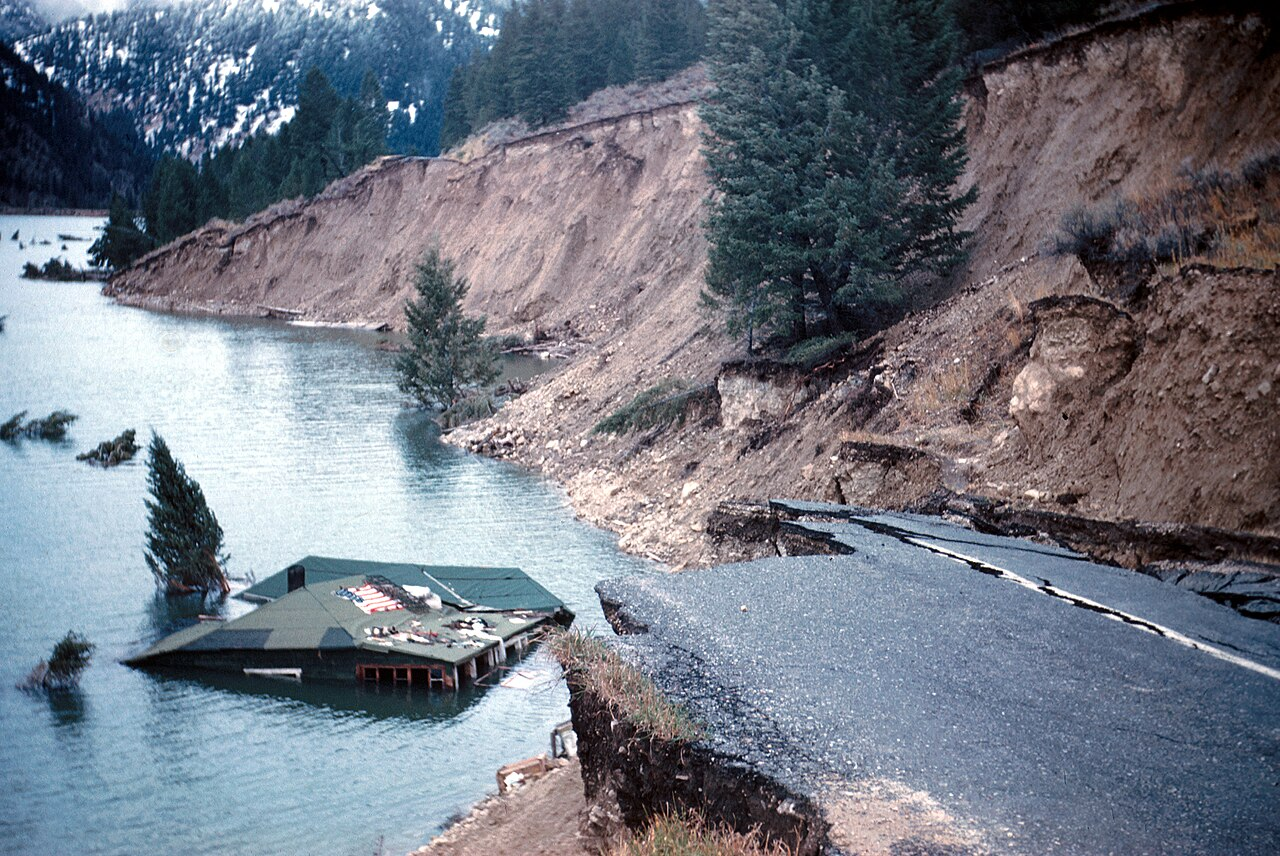
\includegraphics[width=0.6\linewidth]{images/book1/g7-hebgen-road.jpg}

{\small Sesudah \omterm{def:g4:volcanoes-earthquakes-first-look:earthquake}{gempa bumi} Hebgen Lake, Montana (Amerika Serikat), Agustus
1959: jalan di sepanjang \omterm{def:g1:landscapes-around-us:water}{danau} ambles ke dalam air, dan sebuah pondok
penginapan hampir terendam. Kerusakan seperti ini adalah tanda \omterm{def:g7:earthquakes:intensity}{intensitas}
yang tinggi. Foto: I.~J. Witkind, U.S. Geological Survey (domain publik,
melalui Wikimedia Commons).}
% ledger: commons:hebgen-road, usgs:mmi
\label{fig:g7:earthquakes:hebgen}
\end{omfigure}

\section{Tsunami}

\begin{definition}[Tsunami]\label{def:g7:earthquakes:tsunami}
Yang disebut \emph{tsunami}\index{tsunami} adalah serangkaian gelombang \omterm{def:g2:water-on-earth:ocean}{laut}
yang dipicu oleh gerakan dasar \omterm{def:g2:water-on-earth:ocean}{laut} yang tiba-tiba --- biasanya \omterm{def:g4:volcanoes-earthquakes-first-look:earthquake}{gempa bumi}
di bawah \omterm{def:g2:water-on-earth:ocean}{laut}, kadang-kadang \omterm{def:g4:volcanoes-earthquakes-first-look:eruption}{letusan} \omterm{def:g4:volcanoes-earthquakes-first-look:volcano}{gunung api} --- yang dapat menyeberangi
seluruh \omterm{def:g2:water-on-earth:ocean}{samudra} dan membanjiri pantai.
\end{definition}

Ketika sebuah \omterm{def:g7:earthquakes:fault}{sesar} di bawah \omterm{def:g2:water-on-earth:ocean}{laut} patah, dasar \omterm{def:g2:water-on-earth:ocean}{laut} tiba-tiba bergerak naik
atau turun, dan mengangkat atau menurunkan seluruh kolom air di atasnya. Air itu menyebar dalam bentuk gelombang. Di \omterm{def:g2:water-on-earth:ocean}{samudra} yang dalam,
\omterm{def:g7:earthquakes:tsunami}{tsunami} itu mengejutkan: tingginya jarang lebih dari satu meter, dan
kapal-kapal bahkan tidak menyadarinya ketika \omterm{def:g7:earthquakes:tsunami}{tsunami} lewat di bawahnya.
Tetapi \omterm{def:g7:earthquakes:tsunami}{tsunami} itu cepat: lebih dari \qty{800}{km/h}, secepat pesawat jet.
Ketika mencapai perairan dangkal di dekat pantai, \omterm{def:g7:earthquakes:tsunami}{tsunami} melambat menjadi
30 atau \qty{50}{km/h} --- masih lebih cepat daripada lari siapa pun --- dan
makin tinggi. Sebagian besar \omterm{def:g7:earthquakes:tsunami}{tsunami} tingginya kurang dari \qty{3}{m} di
pantai; yang terbesar melampaui \qty{30}{m}. Gelombang pertama tidak selalu
yang terbesar, dan gelombang-gelombang itu dapat terus datang selama
berjam-jam.
% ledger: nws:tsunami-speed, nws:tsunami-safety

\begin{omfigure}
\begin{tikzpicture}[font=\small, x=1cm, y=1cm]
  % sea floor profile: deep ocean on the left, shelf and coast on the right
  \fill[omSea!35] (0,0) -- (13.2,0) -- (13.2,-0.2) -- (11.4,-0.45) -- (10.2,-1.0) -- (8.8,-2.6) -- (0,-2.6) -- cycle;
  \fill[brown!35] (0,-2.6) -- (8.8,-2.6) -- (10.2,-1.0) -- (11.4,-0.45) -- (13.2,-0.2) -- (13.2,0.5) -- (14.2,1.0) -- (14.2,-3.3) -- (0,-3.3) -- cycle;
  % the broken fault under the sea, at left; one block lifted
  \draw[very thick, red!70!black] (1.9,-3.3) -- (2.3,-2.6);
  \draw[-{Stealth[length=2mm]}, thick] (2.75,-3.1) -- (2.75,-2.75);
  \node[anchor=north west, font=\footnotesize, red!70!black] at (0.1,-3.35) {sesar patah, dasar laut terlonjak};
  % wave: low and long in the deep ocean, short and tall near the coast
  \draw[blue!70!black, thick] (0,0) .. controls (1.2,0.18) and (2.2,0.18) .. (3.4,0)
     -- (5.0,0) .. controls (5.8,0.12) and (6.6,0.12) .. (7.4,0) -- (10.6,0)
     .. controls (11.0,0.55) and (11.6,0.9) .. (12.1,0) -- (13.2,0);
  \node[align=center, font=\footnotesize] at (2.0,0.85) {samudra dalam: tinggi kira-kira 1 m,\\lebih dari 800 km/h};
  \node[align=center, font=\footnotesize] at (11.1,1.55) {dekat pantai: lebih lambat\\(30 sampai 50 km/h), jauh lebih tinggi};
  \draw[-{Stealth[length=2.5mm]}, thick, blue!70!black] (4.4,0.45) -- (6.4,0.45);
  \node[font=\footnotesize] at (6.0,-1.5) {dalamnya ribuan meter};
  \node[font=\footnotesize] at (12.0,-0.75) {dangkal};
\end{tikzpicture}

{\small \omterm{def:g7:earthquakes:tsunami}{Tsunami} yang menyeberangi \omterm{def:g2:water-on-earth:ocean}{samudra} (gambar, tidak berskala: tinggi
gelombangnya sangat dilebih-lebihkan). Di atas \omterm{def:g2:water-on-earth:ocean}{samudra} yang dalam, \omterm{def:g7:earthquakes:tsunami}{tsunami}
itu rendah dan sangat cepat; di perairan dangkal di dekat pantai, \omterm{def:g7:earthquakes:tsunami}{tsunami}
itu melambat dan makin tinggi.}
% ledger: nws:tsunami-speed
\label{fig:g7:earthquakes:tsunami}
\end{omfigure}

\begin{example}[Dari Sumatra ke Sri Lanka]\label{ex:g7:earthquakes:colombo}
Kolombo, kota terbesar di Sri Lanka, terletak kira-kira \qty{1830}{km} dari
\omterm{def:g7:earthquakes:focus}{episentrum} \omterm{def:g4:volcanoes-earthquakes-first-look:earthquake}{gempa bumi} tahun 2004. Dengan kecepatan \qty{800}{km/h}, \omterm{def:g7:earthquakes:tsunami}{tsunami}
menempuh jarak ini dalam $1830 \div 800 \approx 2.3$~jam, yaitu kira-kira
2~jam 17~menit. Tidak seorang pun di Sri Lanka merasakan \omterm{def:g4:volcanoes-earthquakes-first-look:earthquake}{gempa bumi} itu:
gelombang itu datang tanpa peringatan apa pun selain dari \omterm{def:g2:water-on-earth:ocean}{laut} itu sendiri.
% ledger: nws:tsunami-speed, usgs:largest (distance and time in figdata/grade-7/quake_counts.py, part tsunami)
\end{example}

\begin{remark}[Peringatan yang diberikan laut]\label{rem:g7:earthquakes:natural-warning}
% ledger: nws:tsunami-natural-warning, nws:tsunami-speed, shakeout:dch
Di pantai, tiga tanda dapat mengabarkan datangnya \omterm{def:g7:earthquakes:tsunami}{tsunami}: \omterm{def:g4:volcanoes-earthquakes-first-look:earthquake}{gempa bumi} yang
kuat atau lama; \omterm{def:g2:water-on-earth:ocean}{laut} yang berperilaku aneh --- \omterm{def:g5:water-shapes-the-land:flood}{banjir} yang tiba-tiba, atau
air yang surut jauh dari pantai sehingga dasar \omterm{def:g2:water-on-earth:ocean}{laut} terlihat seperti saat
air surut yang sangat rendah; atau gemuruh keras yang datang dari \omterm{def:g2:water-on-earth:ocean}{samudra}.
Selama guncangan, lindungilah dirimu seperti yang sudah kamu pelajari
(berlutut, berlindung, berpegangan). Lalu jangan menunggu peringatan resmi:
segera pergilah setinggi mungkin, atau sejauh mungkin ke pedalaman.
\omterm{def:g7:earthquakes:tsunami}{Tsunami} dari \omterm{def:g4:volcanoes-earthquakes-first-look:earthquake}{gempa bumi} yang dekat dapat tiba dalam beberapa menit.
\end{remark}


\section{Latihan}

\begin{exercise}[$\star$]\label{exo:g7:earthquakes:1}
Pasangkan setiap kata dengan artinya: \omterm{def:g7:earthquakes:fault}{sesar}; \omterm{def:g7:earthquakes:focus}{hiposentrum}; \omterm{def:g7:earthquakes:focus}{episentrum};
\omterm{def:g7:earthquakes:seismometer}{seismometer}; \omterm{def:g7:earthquakes:magnitude}{magnitudo}; \omterm{def:g7:earthquakes:intensity}{intensitas}. (a) Tempat di bawah tanah tempat
pergeseran dimulai. (b) Seberapa kuat tanah berguncang di suatu tempat.
(c) Rekahan pada \omterm{def:g3:stones-pebbles-sand:rock}{batuan} yang di sepanjangnya kedua sisinya telah bergerak.
(d) Titik di permukaan di atas \omterm{def:g7:earthquakes:focus}{hiposentrum}. (e) Besarnya \omterm{def:g4:volcanoes-earthquakes-first-look:earthquake}{gempa bumi}, satu
bilangan untuk setiap \omterm{def:g4:volcanoes-earthquakes-first-look:earthquake}{gempa bumi}. (f) Alat yang merekam guncangan tanah.
\end{exercise}

\begin{exercise}[$\star$]\label{exo:g7:earthquakes:2}
\omterm{def:g7:earthquakes:focus}{Hiposentrum} sebuah \omterm{def:g4:volcanoes-earthquakes-first-look:earthquake}{gempa bumi} terletak \qty{30}{km} tepat di bawah sebuah
desa. (a) Di mana \omterm{def:g7:earthquakes:focus}{episentrumnya}? (b) Seberapa jauh desa itu dari
\omterm{def:g7:earthquakes:focus}{hiposentrum}? (c) Desa kedua terletak \qty{40}{km} dari \omterm{def:g7:earthquakes:focus}{episentrum}. Apakah
\omterm{def:g7:earthquakes:intensity}{intensitas} di sana biasanya lebih tinggi atau lebih rendah daripada di
desa pertama? Mengapa?
\end{exercise}

\begin{exercise}[$\star$]\label{exo:g7:earthquakes:3}
\omterm{def:g7:earthquakes:magnitude}{Magnitudo} atau \omterm{def:g7:earthquakes:intensity}{intensitas}? (a) ``\omterm{def:g4:volcanoes-earthquakes-first-look:earthquake}{Gempa bumi} itu berkekuatan 6.8.'' (b) ``Di
jalan kami, semua piring jatuh dan sebuah cerobong patah.'' (c) ``Di kota
nilainya VI dan di desa-desa di perbukitan IV.'' (d) ``Gempa itu
melepaskan energi 32~kali lebih banyak daripada gempa tahun lalu.''
\end{exercise}

\begin{exercise}[$\star$]\label{exo:g7:earthquakes:4}
Benar atau salah? Perbaikilah pernyataan yang salah. (a) Para ilmuwan dapat
mengetahui seminggu sebelumnya kapan \omterm{def:g4:volcanoes-earthquakes-first-look:earthquake}{gempa bumi} akan terjadi. (b) Di
\omterm{def:g2:water-on-earth:ocean}{samudra} lepas, \omterm{def:g7:earthquakes:tsunami}{tsunami} adalah dinding air yang sangat besar. (c) Satu \omterm{def:g4:volcanoes-earthquakes-first-look:earthquake}{gempa
bumi} mempunyai satu \omterm{def:g7:earthquakes:magnitude}{magnitudo} saja tetapi banyak \omterm{def:g7:earthquakes:intensity}{intensitas}. (d) Sebagian
besar \omterm{def:g4:volcanoes-earthquakes-first-look:earthquake}{gempa bumi} besar terjadi di dekat \omterm{def:g7:plate-tectonics:plate-boundary}{batas lempeng}.
\end{exercise}

\begin{exercise}[$\star\star$]\label{exo:g7:earthquakes:5}
Gunakan diagram \omterm{def:g4:volcanoes-earthquakes-first-look:earthquake}{gempa bumi} per tahun. (a) Kira-kira berapa banyak \omterm{def:g4:volcanoes-earthquakes-first-look:earthquake}{gempa
bumi} \omterm{def:g7:earthquakes:magnitude}{bermagnitudo} 6 sampai 6.9 yang terjadi dalam setahun? Yang
\omterm{def:g7:earthquakes:magnitude}{bermagnitudo} 7 sampai 7.9? (b) Berapa kali lebih sedikit yang kedua
dibandingkan dengan yang pertama? (c) Jumlahkan ketiga batang mulai dari 7
ke atas: kira-kira berapa banyak \omterm{def:g4:volcanoes-earthquakes-first-look:earthquake}{gempa bumi} \omterm{def:g7:earthquakes:magnitude}{bermagnitudo} 7 atau lebih yang
terjadi dalam setahun? (d) Diagram itu menunjukkan 0.04 per tahun untuk
\omterm{def:g7:earthquakes:magnitude}{magnitudo} 9 atau lebih. Berapa banyak itu dalam 50~tahun?
\end{exercise}

\begin{exercise}[$\star\star$]\label{exo:g7:earthquakes:6}
Gunakan metode untuk membandingkan \omterm{def:g7:earthquakes:magnitude}{magnitudo}. (a) Berapa kali lebih banyak
energi yang dilepaskan \omterm{def:g4:volcanoes-earthquakes-first-look:earthquake}{gempa bumi} \omterm{def:g7:earthquakes:magnitude}{bermagnitudo} 7 daripada gempa
\omterm{def:g7:earthquakes:magnitude}{bermagnitudo} 6? (b) Dan gempa \omterm{def:g7:earthquakes:magnitude}{bermagnitudo} 8 daripada gempa \omterm{def:g7:earthquakes:magnitude}{bermagnitudo} 6?
(c) Berapa kali lebih besar gelombangnya pada \omterm{def:g7:earthquakes:seismometer}{seismogram}, untuk jarak yang
sama, antara \omterm{def:g7:earthquakes:magnitude}{magnitudo} 6 dan 8?
\end{exercise}

\begin{exercise}[$\star\star$]\label{exo:g7:earthquakes:7}
Gunakan \qty{8}{km} untuk setiap detik selisih antara gelombang yang lebih
cepat dan yang lebih lambat. (a) Sebuah stasiun mencatat selisih
\qty{5}{s}. Seberapa jauh \omterm{def:g4:volcanoes-earthquakes-first-look:earthquake}{gempa bumi} itu? (b) Stasiun lain mencatat
\qty{25}{s}. (c) Sebuah \omterm{def:g4:volcanoes-earthquakes-first-look:earthquake}{gempa bumi} terjadi \qty{120}{km} dari sebuah
stasiun: berapa selisih yang akan dibaca stasiun itu? (d) Mengapa satu
stasiun saja tidak dapat menunjukkan letak \omterm{def:g7:earthquakes:focus}{episentrum}?
\end{exercise}

\begin{exercise}[$\star\star$]\label{exo:g7:earthquakes:8}
Gunakan tabel \omterm{def:g7:earthquakes:intensity}{intensitas}. Tentukan \omterm{def:g7:earthquakes:intensity}{intensitas} untuk setiap laporan.
(a) ``Dirasakan hampir semua orang; kami terbangun dan dua gelas pecah.''
(b) ``Hanya nenekku, yang sedang beristirahat di lantai atas, yang
merasakannya; lampunya berayun.'' (c) ``Dinding dan cerobong roboh;
beberapa rumah runtuh sebagian.'' (d) \omterm{def:g4:volcanoes-earthquakes-first-look:earthquake}{Gempa bumi} yang sama menghasilkan
laporan (a) dan (c). Jelaskan bagaimana hal ini mungkin.
\end{exercise}

\begin{exercise}[$\star\star$]\label{exo:g7:earthquakes:9}
Dari 7\,031 \omterm{def:g4:volcanoes-earthquakes-first-look:earthquake}{gempa bumi} \omterm{def:g7:earthquakes:magnitude}{bermagnitudo}~6 atau lebih pada tahun 1976--2025,
5\,561 \omterm{def:g7:earthquakes:focus}{hiposentrumnya} kurang dari \qty{70}{km} di bawah permukaan.
(a) Berapa banyak yang \omterm{def:g7:earthquakes:focus}{hiposentrumnya} lebih dalam? (b) Berapa persen itu?
Bulatkan ke bilangan bulat terdekat. (c) Gempa-gempa yang dalam terjadi di
tempat satu \omterm{def:g7:plate-tectonics:plate}{lempeng} menunjam ke bawah \omterm{def:g7:plate-tectonics:plate}{lempeng} lain. Jelaskan mengapa
gempa-gempa itu dapat dimulai sedalam itu di sana.
\end{exercise}

\begin{exercise}[$\star\star$]\label{exo:g7:earthquakes:10}
Male, ibu kota Maladewa, terletak kira-kira \qty{2500}{km} dari \omterm{def:g7:earthquakes:focus}{episentrum}
\omterm{def:g4:volcanoes-earthquakes-first-look:earthquake}{gempa bumi} tahun 2004. (a) Dengan kecepatan \qty{800}{km/h}, berapa lama
waktu yang diperlukan \omterm{def:g7:earthquakes:tsunami}{tsunami} untuk mencapainya? Nyatakan dalam jam dan
menit. (b) Berapa lama lebih lambat \omterm{def:g7:earthquakes:tsunami}{tsunami} itu tiba dibandingkan di
Kolombo (2~jam 17~menit)? (c) Dengan selisih waktu seperti itu, mengapa
sistem peringatan dapat menyelamatkan banyak nyawa?
\end{exercise}

\begin{exercise}[$\star\star\star$]\label{exo:g7:earthquakes:11}
Sebuah \omterm{def:g7:earthquakes:tsunami}{tsunami} menyeberangi \omterm{def:g2:water-on-earth:ocean}{samudra} dalam sejauh \qty{400}{km} dengan
kecepatan \qty{800}{km/h}, lalu \qty{20}{km} terakhir di perairan dangkal
dengan kecepatan \qty{40}{km/h}. (a) Berapa menit yang diperlukannya untuk
bagian yang dalam? (b) Untuk bagian yang dangkal? (c) Berapa lama seluruh
perjalanannya? (d) Apa yang mengejutkan dalam jawabanmu? (e) Mengapa
gelombang itu makin tinggi ketika melambat?
\end{exercise}

\begin{exercise}[$\star\star\star$]\label{exo:g7:earthquakes:12}
(a) Berapa kali lebih banyak energi yang dilepaskan \omterm{def:g4:volcanoes-earthquakes-first-look:earthquake}{gempa bumi} \omterm{def:g7:earthquakes:magnitude}{bermagnitudo}
9 daripada gempa \omterm{def:g7:earthquakes:magnitude}{bermagnitudo} 6? (b) Setiap tahun terjadi kira-kira 127
\omterm{def:g4:volcanoes-earthquakes-first-look:earthquake}{gempa bumi} \omterm{def:g7:earthquakes:magnitude}{bermagnitudo} 6 sampai 6.9. Andaikan masing-masing melepaskan
energi gempa \omterm{def:g7:earthquakes:magnitude}{bermagnitudo} 6. Berapa tahun gempa-gempa seperti itu yang
diperlukan untuk melepaskan energi satu \omterm{def:g4:volcanoes-earthquakes-first-look:earthquake}{gempa bumi} \omterm{def:g7:earthquakes:magnitude}{bermagnitudo}~9? (c) Apa
yang ditunjukkan hal ini tentang bagian energi yang dibawa oleh gempa-gempa
bumi yang paling besar?
\end{exercise}

\section{Soal: Di mana tanah berguncang?}

\begin{problem}[{Soal akhir pekan --- tiga stasiun merekam gempa bumi di
bawah laut, episentrumnya ditemukan pada peta, dan kota Port Hale diberi
peringatan sebelum tsunami tiba}]
\label{pb:g7:earthquakes:1}
% ledger: nws:tsunami-speed, usgs:seismograph, data:prem (figdata/grade-7/epicentre.py)
Sebuah \omterm{def:g4:volcanoes-earthquakes-first-look:earthquake}{gempa bumi} terjadi di bawah \omterm{def:g2:water-on-earth:ocean}{laut} di sebuah pantai rekaan. Tiga
stasiun \omterm{def:g7:earthquakes:seismometer}{seismometer}, A, B, dan C, terletak di darat; kota Port Hale
terletak di sebuah pulau (\omterm{def:g2:drawing-to-map:map}{peta} di bawah; satu kotak = \qty{20}{km}). Di
wilayah ini, setiap detik selisih antara gelombang yang lebih cepat dan
yang lebih lambat berarti \qty{8}{km}. Stasiun-stasiun itu mencatat:

\begin{center}
\small
\begin{tabular}{|c|c|c|}
\hline
\textbf{stasiun} & \textbf{gelombang yang lebih cepat tiba} & \textbf{gelombang yang lebih lambat tiba} \\
\hline
A & 10.15.25 & 10.15.45 \\
B & 10.15.16 & 10.15.29 \\
C & 10.15.19 & 10.15.34 \\
\hline
\end{tabular}
\end{center}

\medskip
\noindent\textbf{Bagian I --- Tiga stasiun.}\par\nopagebreak
\begin{enumerate}[beginpenalty=10000]
  \item Untuk setiap stasiun, tentukan selisih waktu antara kedua
        kedatangan, dalam detik.
  \item Stasiun mana yang paling dekat dengan \omterm{def:g4:volcanoes-earthquakes-first-look:earthquake}{gempa bumi}? Bagaimana kamu
        dapat mengetahuinya tanpa menghitung apa pun?
  \item Tentukan jarak dari setiap stasiun ke \omterm{def:g4:volcanoes-earthquakes-first-look:earthquake}{gempa bumi}.
  \item Jarak stasiun A saja tidak menunjukkan di mana \omterm{def:g4:volcanoes-earthquakes-first-look:earthquake}{gempa bumi} itu.
        Jelaskan semua tempat yang berjarak sejauh itu dari A.
\end{enumerate}

\begin{center}
\begin{tikzpicture}
  \begin{axis}[axis equal image, width=12cm, xmin=-60, xmax=360, ymin=-200, ymax=260,
      xtick={-60,-40,...,360}, ytick={-200,-180,...,260}, xticklabels={}, yticklabels={},
      major tick length=0pt,
      axis background/.style={fill=omSea!25}, clip mode=individual]
    \addplot[fill=omLithAlluv, draw=black!50, line width=0.4pt] table[x=x, y=y] {figdata/out/grade-7-epicentre-p-west.dat};
    \addplot[fill=omLithAlluv, draw=black!50, line width=0.4pt] table[x=x, y=y] {figdata/out/grade-7-epicentre-p-north.dat};
    \addplot[fill=omLithAlluv, draw=black!50, line width=0.4pt] table[x=x, y=y] {figdata/out/grade-7-epicentre-p-island.dat};
    % the grid over land and sea, drawn before the labels
    \pgfplotsinvokeforeach{-40,-20,...,340}{\draw[black!15] (axis cs:#1,-200) -- (axis cs:#1,260);}
    \pgfplotsinvokeforeach{-180,-160,...,240}{\draw[black!15] (axis cs:-60,#1) -- (axis cs:360,#1);}
    \addplot[only marks, mark=triangle*, mark size=3.2pt, black,
        nodes near coords, point meta=explicit symbolic,
        nodes near coords style={font=\small\bfseries, anchor=south west}]
      table[x=x, y=y, meta=name] {figdata/out/grade-7-epicentre-p-stations.dat};
    \addplot[only marks, mark=square*, mark size=2.4pt, red!70!black,
        nodes near coords, point meta=explicit symbolic,
        nodes near coords style={font=\small, anchor=north east, fill=omSea!25, inner sep=1pt}]
      table[x=x, y=y, meta=name] {figdata/out/grade-7-epicentre-p-town.dat};
    \draw[-{Stealth[length=2.5mm]}, line width=0.8pt] (axis cs:330,200) -- (axis cs:330,245);
    \node[font=\scriptsize\bfseries, anchor=north] at (axis cs:330,200) {U};
    \node[font=\scriptsize, anchor=west, fill=omLithAlluv, inner sep=1pt] at (axis cs:170,240) {1 kotak = 20 km};
    \fill (axis cs:-60,-200) circle (1.5pt);
    \node[font=\small\bfseries, anchor=north east] at (axis cs:-60,-200) {O};
  \end{axis}
\end{tikzpicture}
\end{center}
% ledger: (invented map: figdata/grade-7/epicentre.py, parts p-west, p-north, p-island, p-stations, p-town)

\medskip
\noindent\textbf{Bagian II --- Menemukan episentrum.}\par\nopagebreak
\begin{enumerate}[resume, beginpenalty=10000]
  \item Satu kotak = \qty{20}{km}. Berapa kotak jari-jari setiap
        lingkaran?
  \item Letakkan titik sudut O di kiri bawah \omterm{def:g2:drawing-to-map:map}{peta}. Stasiun C terletak
        3~kotak ke timur dan 14.5~kotak ke utara dari O; jika kamu berjalan
        6~kotak (\qty{120}{km}) lurus ke timur dari C, kamu sampai di
        titik~E. Periksalah pada \omterm{def:g2:drawing-to-map:map}{peta} bahwa E juga terletak pada lingkaran A
        dan lingkaran B: itulah \omterm{def:g7:earthquakes:focus}{episentrumnya}. Berapa kotak ke timur dan ke
        utara dari O letaknya?
  \item Apakah \omterm{def:g7:earthquakes:focus}{episentrum} itu di darat atau di bawah \omterm{def:g2:water-on-earth:ocean}{laut}? Mengapa hal itu
        penting?
  \item \omterm{def:g7:earthquakes:magnitude}{Magnitudonya} 7.4. Berapa kali lebih banyak energi yang
        dilepaskannya daripada \omterm{def:g4:volcanoes-earthquakes-first-look:earthquake}{gempa bumi} \omterm{def:g7:earthquakes:magnitude}{bermagnitudo}~6.4?
\end{enumerate}

\medskip
\noindent\textbf{Bagian III --- Gelombang mencapai pantai.}\par\nopagebreak
\begin{enumerate}[resume, beginpenalty=10000]
  \item Pada \omterm{def:g2:drawing-to-map:map}{peta}, Port Hale berjarak 12~kotak dari \omterm{def:g7:earthquakes:focus}{episentrum}. Berapa
        kilometer itu?
  \item Dengan kecepatan \qty{800}{km/h}, berapa menit yang diperlukan
        \omterm{def:g7:earthquakes:tsunami}{tsunami} untuk mencapai Port Hale?
  \item Menentukan letak \omterm{def:g4:volcanoes-earthquakes-first-look:earthquake}{gempa bumi} dan mengirimkan peringatan memerlukan
        waktu 5~menit sesudah guncangan dimulai. Berapa menit sesudah \omterm{def:g4:volcanoes-earthquakes-first-look:earthquake}{gempa
        bumi} peringatan itu sampai di Port Hale?
  \item Berapa menit yang dimiliki penduduk Port Hale untuk mencapai tempat
        yang tinggi sebelum \omterm{def:g7:earthquakes:tsunami}{tsunami} tiba?
\end{enumerate}
\end{problem}
